\documentclass[10pt]{article}
\usepackage[letterpaper,margin=0.62in]{geometry}
\usepackage{booktabs,graphicx,wrapfig,enumitem,xcolor,microtype}
\usepackage[hidelinks]{hyperref}
\setlist{nosep,leftmargin=1.2em}
\setlength{\parskip}{2pt}\setlength{\parindent}{0pt}
\renewcommand{\arraystretch}{0.95}
\newcommand{\sect}[1]{\vspace{3pt}{\large\bfseries #1}\par\vspace{1pt}}
% GitHub URL
\newcommand{\repo}{\url{https://github.com/areddy75/Computer-Vision-Assignment-1}}

\begin{document}
\begin{center}
{\Large\bfseries ITCS 6169/8169 Assignment 1 --- The CNN Challenge}\\[1pt]
Anusha Reddy \quad$\cdot$\quad Code, configs, logs \& final checkpoint: \repo
\end{center}

\sect{1. Final result}
\textbf{Test accuracy: 96.75\,\% (387/400)} with a single fine-tuned \textbf{ConvNeXt-Tiny} CNN.
\textbf{Validation strategy:} stratified 80/20 split of the 2,400 training images (120/30 per class, seed 0), identical for every experiment; model selection = epoch with the best validation accuracy. The test set was evaluated \emph{once}, after the final model had been chosen on validation and that choice committed to git.
\textbf{Validation accuracy of the selected model: 96.67\,\% (464/480)}; the test number agrees to within one image.
Reproduce: \texttt{python train.py --config configs/best.yaml}; \texttt{python evaluate.py --checkpoint checkpoints/final\_convnext\_tiny\_fp16.pt}.

\sect{2. The recipe, and which choices mattered}
\begin{wrapfigure}{r}{0.45\textwidth}
\vspace{-14pt}\centering
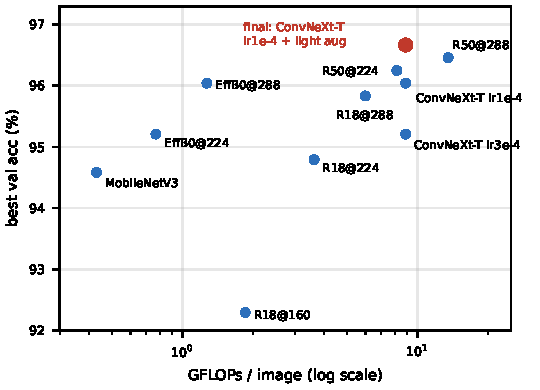
\includegraphics[width=0.45\textwidth]{acc_vs_flops.pdf}
\vspace{-6pt}
\parbox{0.45\textwidth}{\centering\footnotesize Fig.\,1: val accuracy vs.\ compute (ImageNet-pretrained CNNs; R = ResNet).}
\vspace{-8pt}
\end{wrapfigure}
\textbf{Architecture/initialisation:} ConvNeXt-Tiny (28\,M params) initialised from torchvision \texttt{IMAGENET1K\_V1} weights; the 1000-way head is replaced by a 16-way linear layer and \emph{all} layers are fine-tuned. The 256\,px greyscale images are replicated to 3 channels and normalised with ImageNet statistics; input $224{\times}224$.
\textbf{Optimisation:} AdamW, lr $10^{-4}$, weight decay 0.05 (not on norms/biases), 1 warm-up epoch + cosine decay, batch 32, 30 epochs (40\,min on an Apple M4).
\textbf{Regularisation:} label smoothing 0.1; \emph{light} augmentation only (reflect-pad random crop + horizontal flip). No test-time augmentation (it lowered val accuracy).
\textbf{What mattered, in order:} (1) \emph{ImageNet initialisation} (+5.8\,\% for the same ResNet-18; a frozen-backbone linear probe already beats every from-scratch model); (2) \emph{task-appropriate augmentation}: light $>$ strong by +1.0\,\% (2 seeds); (3) \emph{label smoothing} (+1.5\,\% mean over 3 seeds, every seed improved); (4) the \emph{learning rate} for ConvNeXt (3e-4$\to$1e-4: +0.8\,\%, far more stable curve); (5) \emph{resolution}: 288\,px gave +1.4\,\% for ResNet-18 and +1.1\,\% for EfficientNet-B0. The \emph{CNN family} mattered least: five ImageNet CNNs from 0.4 to 9 GFLOPs land within $\sim$1\,\% of each other (Fig.\,1). \textbf{Efficiency pick:} EfficientNet-B0 @288\,px reaches 96.0\,\% val at 1/7 of the FLOPs.

\sect{3. Experimental journey}
\vspace{-2pt}
{\small
\begin{tabular}{@{}p{0.42\textwidth}r p{0.41\textwidth}@{}}
\toprule
Experiment (one change at a time) & Val acc. & Observation \\ \midrule
Baseline: starter TNet, grey 64\,px & 44.0\,\% & 99\,\% train acc.: overfits, and features too weak \\
Own 8-layer CNN (BN, GAP), 128\,px, AdamW+cosine & 87.7\,\% & depth/GAP head $\gg$ parameter count (1.2\,M) \\
+ strong / \textbf{light} augmentation & 87.3 / 90.2\,\% & strong aug \emph{hurt} (Sec.\,4); light aug helps \\
ResNet-18 from scratch, 224\,px & 86.7\,\% & 10$\times$ the capacity, no gain without pretraining \\
+ ImageNet init (all layers fine-tuned) & 92.9\,\%$^\dagger$ & pretraining is the largest single gain \\
+ label smoothing 0.1 & 94.4\,\%$^\dagger$ & consistent over 3 seeds (std 0.6\,\%) \\
+ MixUp/CutMix & 92.9\,\% & hurt: over-regularises a 30-epoch run \\
+ light instead of strong aug & 95.4\,\%$^\dagger$ & the scratch-model finding transfers \\
Family (224\,px): MobileNetV3, EffNet-B0, ResNet-50, ConvNeXt-T & 94.6--95.7\,\% & 94.6 / 94.9$^\dagger$ / 95.7$^\dagger$ / 95.2\,\%: within $\sim$1\,\% \\
ConvNeXt-T, lr 3e-4$\to$1e-4 & 96.5\,\%$^\dagger$ & lr was limiting ConvNeXt, not capacity \\
\textbf{Final: ConvNeXt-T, lr 1e-4, light aug} & \textbf{96.7\,\%} & \textbf{test 96.75\,\%} \\ \bottomrule
\end{tabular}}\\[1pt]
{\footnotesize $^\dagger$mean over 2--3 training seeds (same split). One val image = 0.21\,\%; single-seed differences $<$1\,\% were treated as noise and re-run.}

\sect{4. Failure analysis: strong augmentation made things worse}
\textbf{What I tried:} the standard ImageNet-style pipeline (RandomResizedCrop with scale 0.35--1, brightness/contrast jitter, $\pm10^\circ$ rotation, flip) on the from-scratch CNN, which was at 100\,\% train accuracy.
\textbf{Why I expected it to work:} augmentation is the usual remedy for overfitting on 1,920 images.
\textbf{What happened:} validation accuracy \emph{dropped} (87.7$\to$87.3\,\%) and train accuracy fell to 90\,\%, with the best epoch being the last. I tested three explanations, one change each: (i) \emph{under-training}: 150 instead of 60 epochs reached 97\,\% train accuracy but only 88.1\,\% val, so convergence was not the problem; (ii) \emph{aggressive crops}: restricting the crop scale to 0.8--1 recovered part of the loss (88.8\,\%); (iii) \emph{only label-preserving geometry} (pad-crop + flip): 90.2\,\%, the best scratch result.
\textbf{What I learned:} scene classes are defined by \emph{global layout} (horizon position, sky/ground ratio, vertical structure). A 35\,\%-area crop of a \emph{Coast} image is plausibly \emph{OpenCountry}, and rotation adds black corners never seen at test time, so the augmented training distribution drifts away from the test distribution instead of covering it. Augmentation must be label-preserving \emph{for the task}. The lesson transferred: light augmentation also improved the pretrained ResNet-18 (+1.0\,\%, 2 seeds) and is part of the final model. Two smaller surprises: MixUp/CutMix hurt (--1.9\,\%), and ResNet-50's first run (96.3\,\%) was partly luck: its best-vs-last-epoch gap was 1.7\,\% and a second seed gave 95.2\,\%.

\textbf{Error analysis.} The hardest classes are consistent across models: \emph{InsideCity} and \emph{Bedroom} (confused with \emph{LivingRoom}) on validation. 9 of the 13 test errors involve \emph{OpenCountry} (e.g.\ grassy hillsides labelled \emph{Mountain}); several are arguably ambiguous labels. Pretraining helped most on \emph{OpenCountry} (+17\,\%) and \emph{Industrial} (+13\,\%), and not at all on \emph{InsideCity}.

\sect{5. AI + Human}
I used \textbf{Claude Code} as a pair programmer (details in \texttt{AI\_USAGE.md}). \textbf{Where it helped:} it turned the starter notebook into a config-driven, logged pipeline in minutes and built a throughput benchmark that located the real bottleneck. \textbf{Where judgement was needed:} its suggested \texttt{channels\_last} speed-up (good advice on CUDA) made training 2--3$\times$ \emph{slower} on the Apple GPU; it was measured and removed. More importantly, a first-draft analysis written before the numbers were checked mis-stated which classes benefit from pretraining. Every claim in this report was re-derived from the logged results, and every decision-driving comparison was repeated with extra seeds before being believed.
% >>> EDIT: replace the last two sentences with your own example of a decision YOU made (see AI_USAGE.md). <<<

\end{document}
